\documentclass[acmtog]{acmart}
\usepackage{graphicx}
\usepackage{subfigure}
\usepackage{natbib}
\usepackage{listings}
\usepackage{bm}
\usepackage{soul}
\usepackage{algorithm}
\usepackage{algorithmic}

\definecolor{blve}{rgb}{0.3372549 , 0.61176471, 0.83921569}
\definecolor{gr33n}{rgb}{0.29019608, 0.7372549, 0.64705882}
\makeatletter
\lst@InstallKeywords k{class}{classstyle}\slshape{classstyle}{}ld
\makeatother
\lstset{language=C++,
	basicstyle=\ttfamily,
	keywordstyle=\color{blve}\ttfamily,
	stringstyle=\color{red}\ttfamily,
	commentstyle=\color{magenta}\ttfamily,
	morecomment=[l][\color{magenta}]{\#},
	classstyle = \bfseries\color{gr33n}, 
	tabsize=2
}
\lstset{basicstyle=\ttfamily}

% Title portion
\title{Assignment 1:\\ {3D Convex Hull Problems}}

\author{Name:\quad Chenqihe  \\ student number:\ 2020533088
\\email:\quad chenqh@shanghaitech.edu.cn}

% Document starts
\begin{document}
\maketitle

\vspace*{2 ex}

\section{Introduction}
	\quad \st{This report only includes HW1 part2. If you want to read part1, please refer to another pdf file in this directory.}
	
	\quad In this assignmment, we complete two tasks. First, we implement a 3D convex hull algorithm with visualization. Second, we implement collision detection for two convex hulls of two 3D point sets. Also, 2nd task is based on the completion of 1st task.
	
	\quad In 1st task, I achieve 3D convex hull construction by 3D version of incremental algorithm, and display the visualization based on OpenGL. By the way, all the frameworks are set up by myself, it takes me about 3 days to complete the frameworks.
	
	\quad In 2nd task, I achieve 3D convex hulls collision detection by 3D version of sparating axis theorem algorithm,  display runtime analysis information and speed up the algorithm by using OpenMP. I believe that I don't make it perfectly since I don't use matrix operation to make use of GPU sources which limits the performance of this algorithm with many dots products.
	
\section{Related work}
In this section, we review related work to provide context for our own work.

\textbf{3D convex hull algorithm} In computational geometry, convex hull is an important concept, which can be used in object compression, collision detection and a varitey of computer graphics scenes. There is a formal definition of convex hull: The Convex Set / Convex Combination for point set $S(p_1, p_2,\cdots, p_n)$ is denoted as 
\[
\sum_{i=1}^n\alpha_ip_i. \quad(\alpha_i\ge 0, \sum_{i=1}^n\alpha_i=1)
\]
\quad The convex hull, convex envelop or convex closure of $S$ is the union of all the convex combinations of $S$.

\textbf{3D collision detection} As shown above, convex hull has lots of application, such as fast collision queries (games, robots), shape matching (convex deficiency trees, similarity analysis... ), serving for other geometric construction (Voronoi...) and many other (building fence for a castle). In this report, we talk about how to use convex hull on 3D collision detection problem.

\textbf{Incremental algorithm} There exists many kinds of algorithms to solve convex hull problems, like extreme edges algorithm, gift wrapping algorithm, quick hull algorithm, graham algorithm, incremental algorithm, divide and conquer algorithm. All six algorithms can be easily achieved on 2D convex hull problems. However, we are faced with convex hull problem in 3D scene, which implies that we have to encounter with much more boundaries problems and floating accuracy error. With really carefully tradeoff between the complexity of the algorithm and the implementation difficulty, we choose incremental algorithm as our solver.

\begin{itemize}
	\item Thanks to modern CPU speed, we can solve 3D convex problem in most common cases in $O(n^2)$ time complexity.
	\item The boundary problems can be easily solved by making a small perturb onto point set. And the floating accuracy error is small enough to negligible.
	\item It allows adding a new point to existing convex hull in $O(n)$ time complexity.
\end{itemize}

\textbf{3D Separating Axis Theorem} There are many ways to solve 3D convex set collision detection problems, such as GJK, SAT and so on. However, most of them work very well on 2D scene, and it is undirect to convert them into 3D scene. Thanks to the power of sparating hyperplane theorem, it provides the basic theory for us to extend SAT algorithm into 3D scene.

\textbf{Separating hyperplane theorem} Let $C$ and $D$ be two convex sets in $R^n$ that do not intersect (i.e., $C\cap D=\emptyset$). Then, there exists $a\in R^n$, $a\not=0, b\in R$, such that $\forall x\in C,\forall y\in D$
$$
a^Tx\le b \text{ and } a^Ty\ge b
$$
	\quad It tells us that in most common cases, we can solve collision detection problems in any dimension if we can find the sparating hyperplane. As for 3D scene with convex sets, we just need to find a spearating plane not a sperating maniforms. Meanwhile, we remark that neither inequality in the conclusion of sparating hyperplane theorem can be made strict. Therefore, we should take boundaries cases into careful consideration later.
\section{Methods}
\subsection{Basic pipeline for task 1}

\begin{figure}[h]
	\centering
	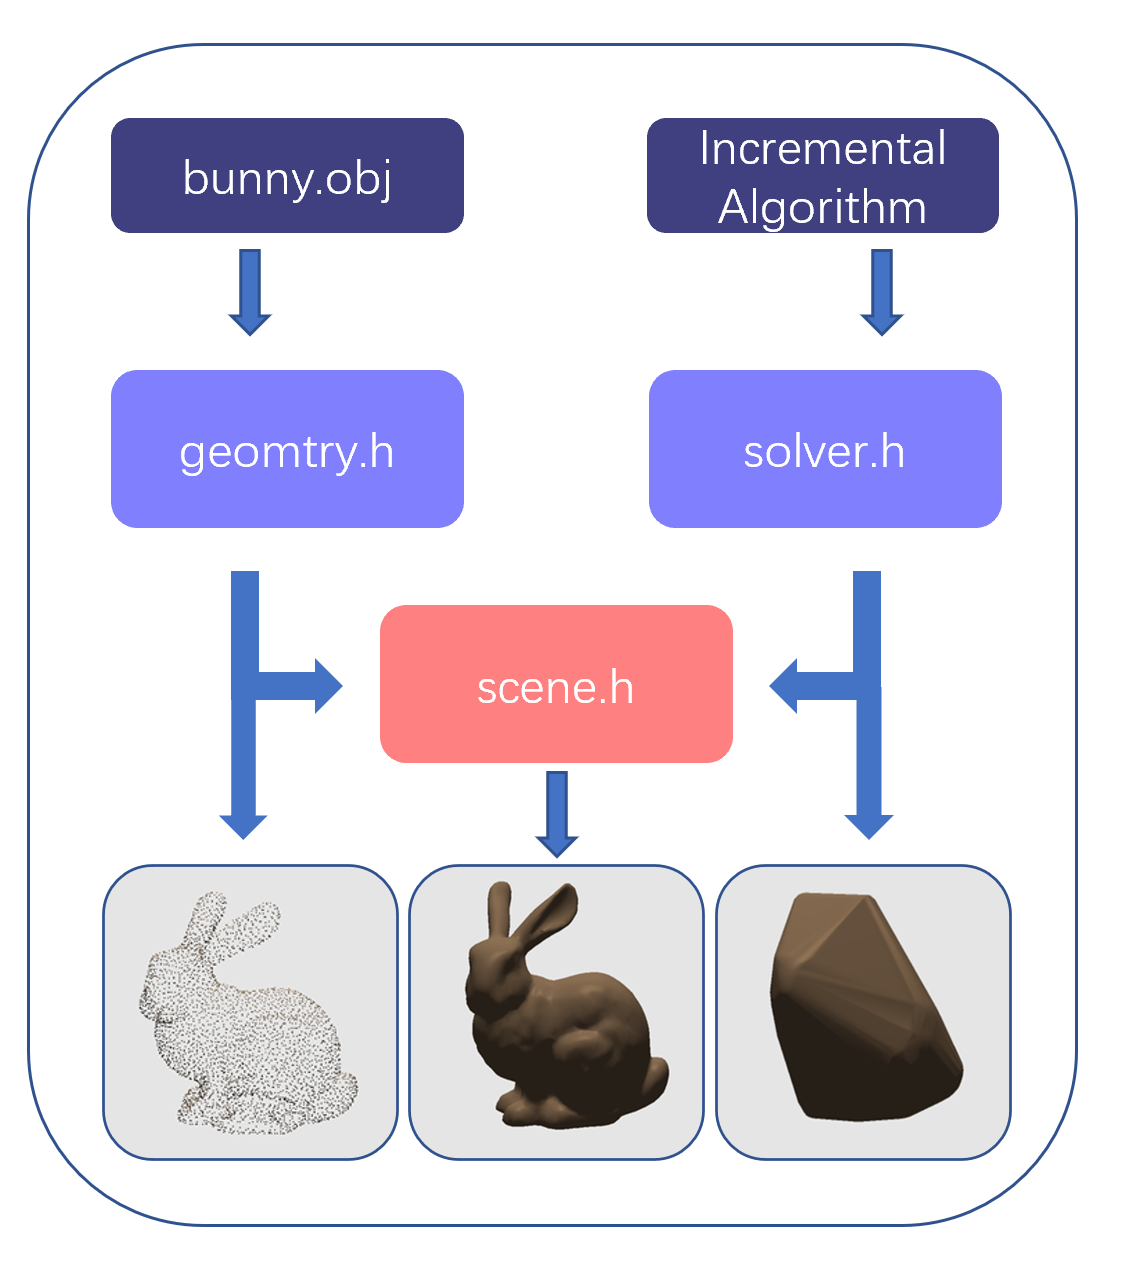
\includegraphics[scale=0.15]{pipeline1.png}
	\caption{Basic pipeline for task 1}
	\label{fig:img1}
\end{figure}
	
	\quad \textbf{Input:} First, we use "obj\_loader.h" to load .obj file and store its vertices, normals and faces w.r.t the indices. Second, we use these data to formulate our geometry in "geometry.h". Third, our scene in "scene.h" has a vector to accommodate all the geometries.
	
	\quad \textbf{Process:} We integrate our incremental algorithm from "solver.h" into our scene in "scene.h". If we receive the signal from input, we process the incremental algorithm onto each geometries in real-time, respectively. 
	
	\quad \textbf{Output:} Based on OpenGL, our scene in "scene.h" can render  in real-time with three modes, point clouds, mesh clouds or convex hull.
	
\subsection{Incremental algorithm}
\begin{figure}[h]
	\centering
	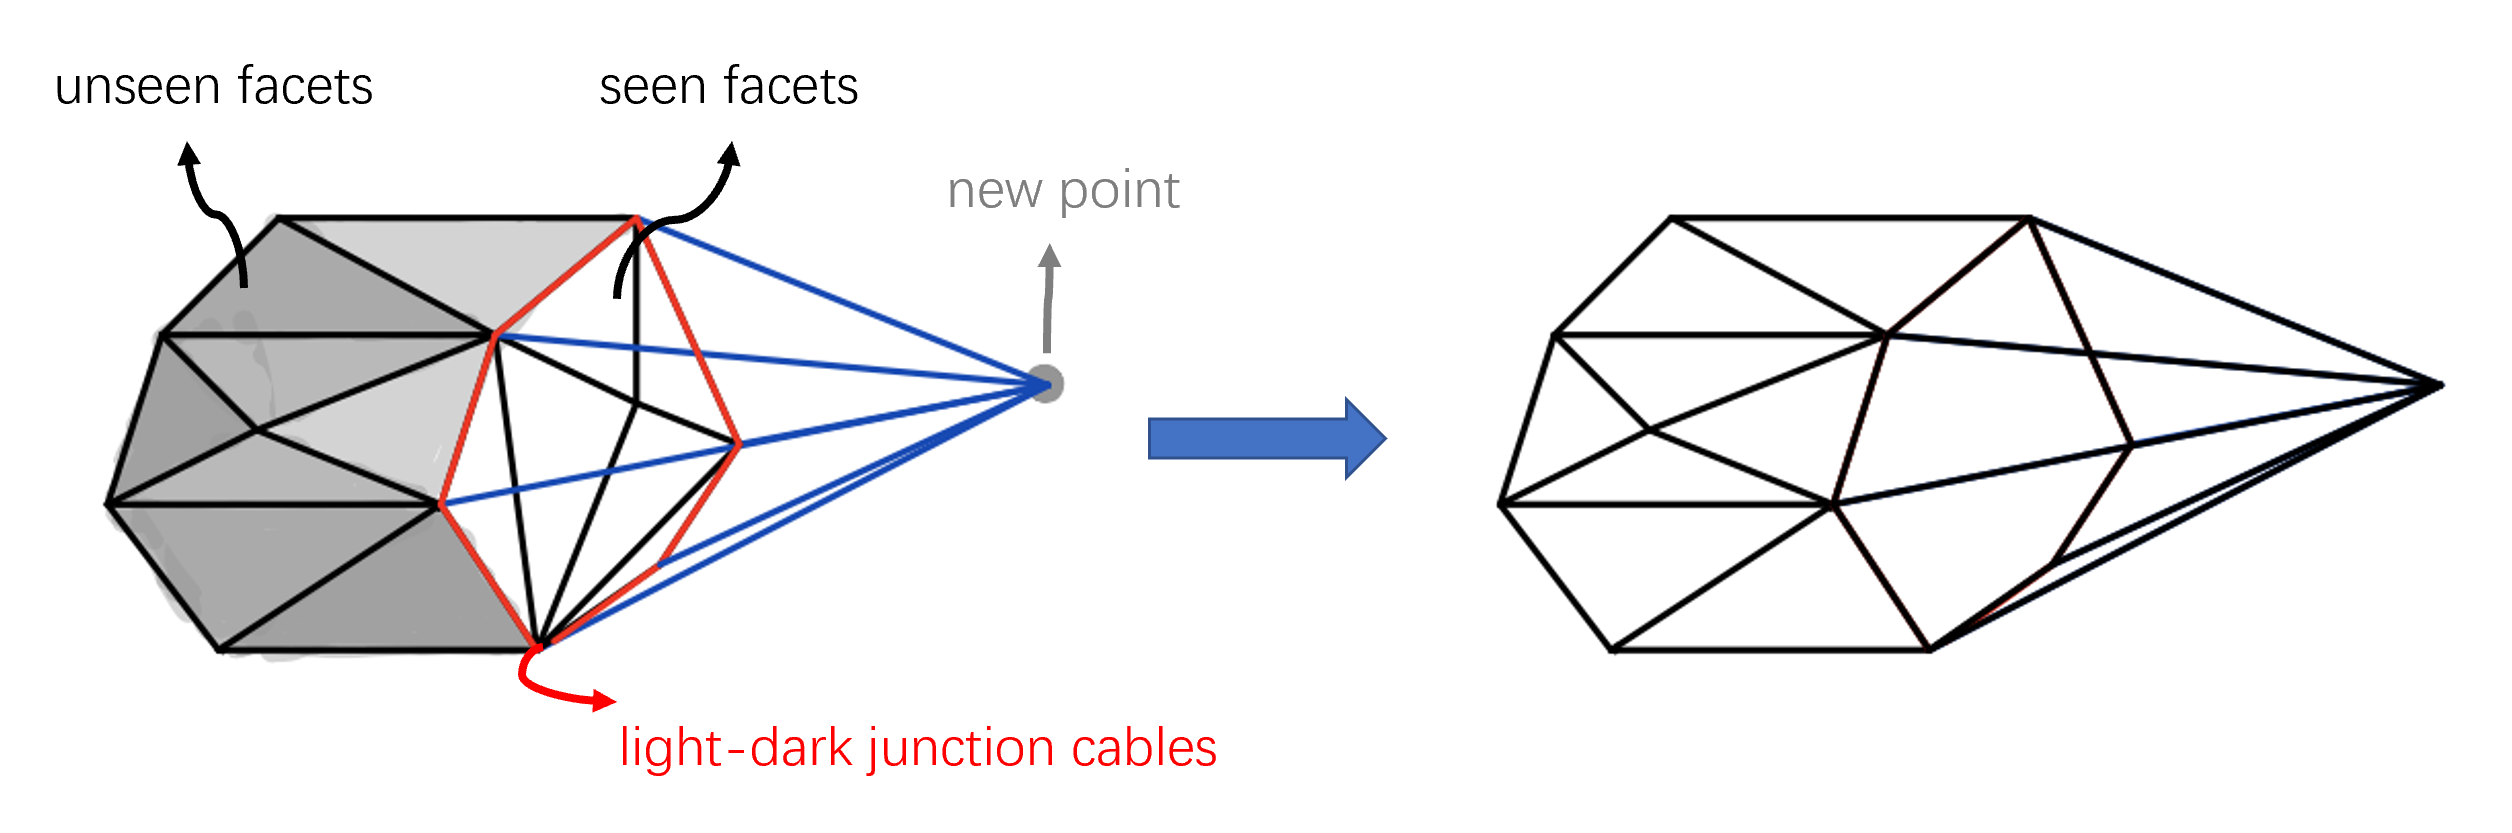
\includegraphics[scale=0.1]{incremental algorithm.png}
	\caption{Incremental algorithm}
	\label{fig:img2}
\end{figure}
	\quad \textbf{Main idea:} For each step, we add a new point into existing convex hull by connecting the new point with the light-dark junction cables, and delete all facets within the region formed by the new faces w.r.t new points and corresponding light-dark junction cables in order.

\begin{algorithm}
	\caption{Incremental algorithm}
	\begin{algorithmic}[1]
		\STATE // small perturb to avoid three points on line
		\STATE vertices $\leftarrow$ perturb(vertices) 
		\STATE // init
		\STATE  convexhull $\leftarrow$ facet$(v_0, v_1, v_2)$, facet$(v_2, v_1, v_0)$
		\FOR{$v \leftarrow $ vertices  // start from $v_4$}
			\STATE // remove all seen facets and find all light-dark junction cables
			\FOR{$f \leftarrow $ convexhull}
				\STATE seen $\leftarrow$ check whether $v$ can see $f$ or not // talk it later
				\IF{seen}
					\STATE convexhull $\leftarrow$ remove $f$ from convexhull
				\ENDIF
			\ENDFOR
			\STATE // adding new facets w.r.t $v$ and found cables
			\FOR{$l \leftarrow$ foundcables}
				\STATE convexhull $\leftarrow$ add facet$(l, i)$
			\ENDFOR
			
		\ENDFOR
		\RETURN  convexhull
	\end{algorithmic}
\end{algorithm}
	
\subsection*{How to check $v$ can see $f$?}
	\quad Specially, since all facets' vertices are in order, the normals (calculate by cross product) always point to the outside of the convexhull. Thus, with perturbing operation at initialization, $v$ can see $f$ if and only if dot product is positive, i.e. 
	\[
	\vec{n} = \vec{p_0p_1} \times \vec{p_0p_2} \Longrightarrow \vec{n} \cdot \vec{p_0v} > 0
	\]

\subsection*{Time complexity analysis}
	\quad First, we need to add vertices one by one, which contributes $O(n)$ time complexity. 
	
	\quad Second, for adding each vertice, we traverse all facets in existing convexhull. The number of convex hull cannot be greater $2n$, since we add at most two new facets more than the deleted-seen facets. 
	
	\quad More objectively, since each triangular area is enclosed by exactly 3 edges, by Euler's formula, we have 
	\[
	f\le 2v -4
	\]
		
	\quad Therefore, for adding each vertice, we also cost $O(n)$ time complexity. To sum up, the total time complexity is $O(n^2)$.
	
\subsection*{Space complexity analysis}
	\quad As talked in time complexity analysis, we need $O(n)$ space complexity to store vertices, and $O(n)$ space complexity to store convexhull. Therefore, the total space complexity is $O(n)$.
	
\subsection{Basic pipeline for task 2}

\begin{figure}[h]
	\centering
	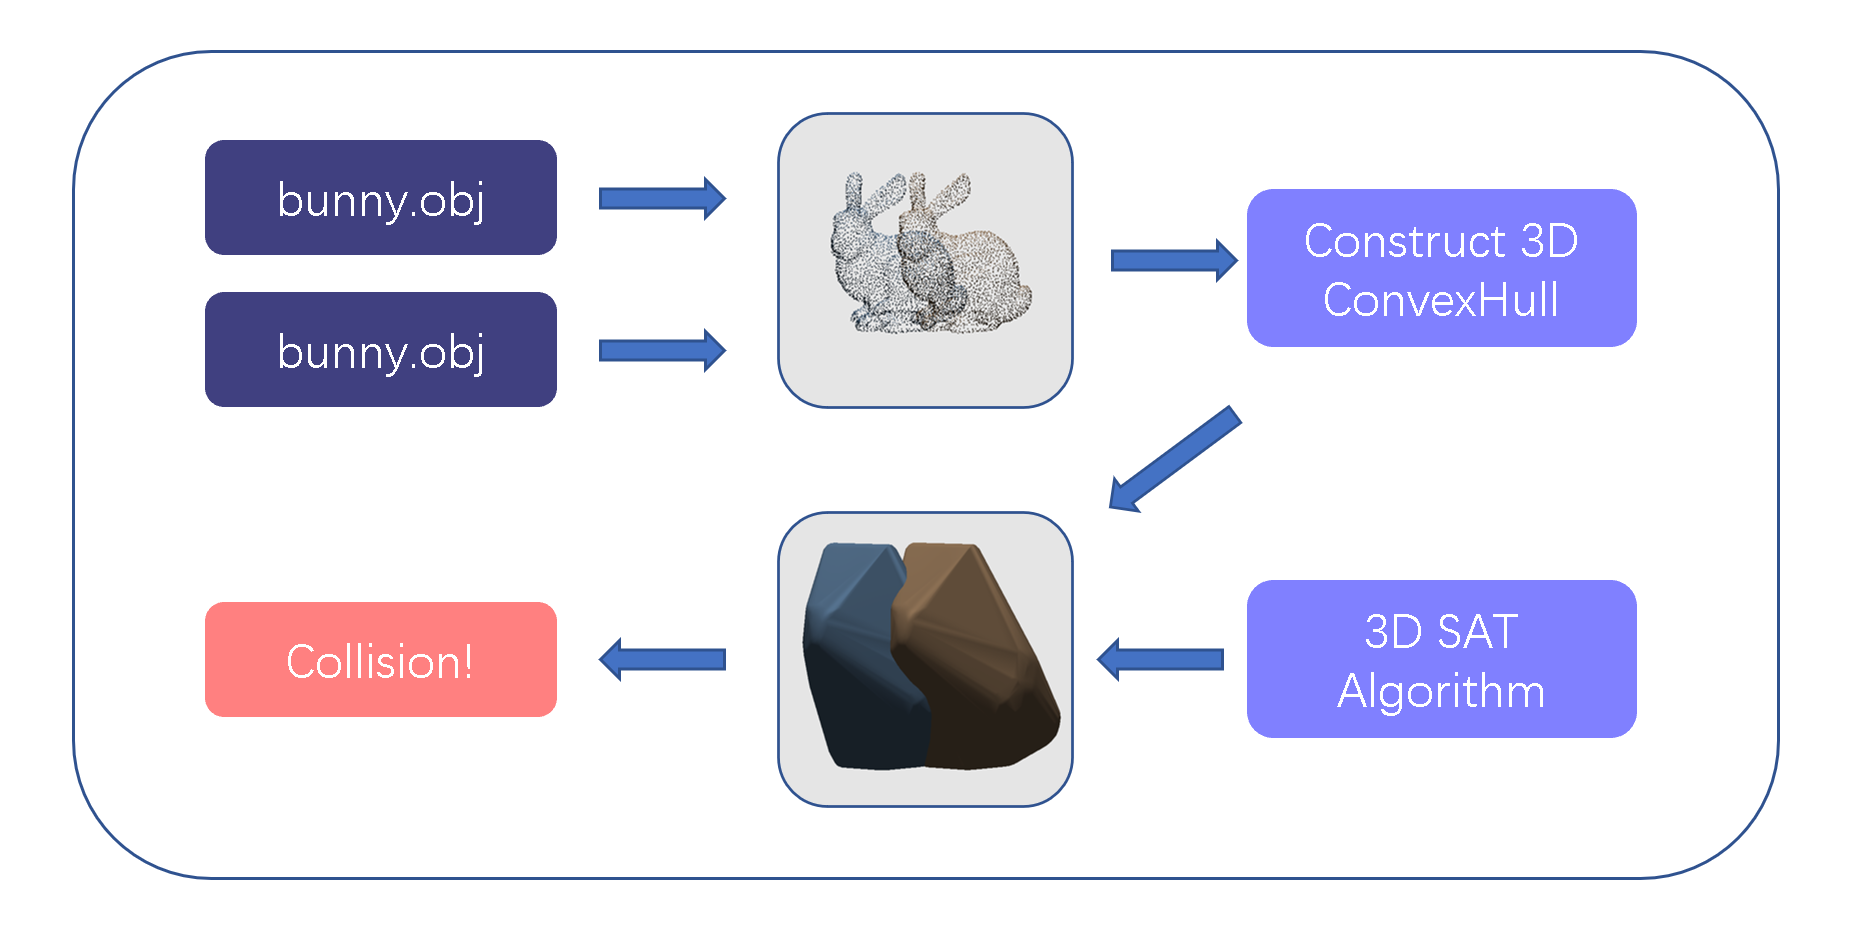
\includegraphics[scale=0.15]{pipeline2.png}
	\caption{Basic pipeline for task 2}
	\label{fig:img3}
\end{figure}

\textbf{Input:} Two convex hulls constructed by task 1.

\textbf{Process:} Using 3D-SAT algorithm to perform the collision detection, and SAT is integrated in our "solver.h".

\textbf{Output:} Solver outputs some information including runtime, data scale and state where we finds the non-collision if not collision. Of course, it outputs whether the collision happens.

\subsection{3D SAT algorithm}
	
	\begin{figure}[h]
		\centering
		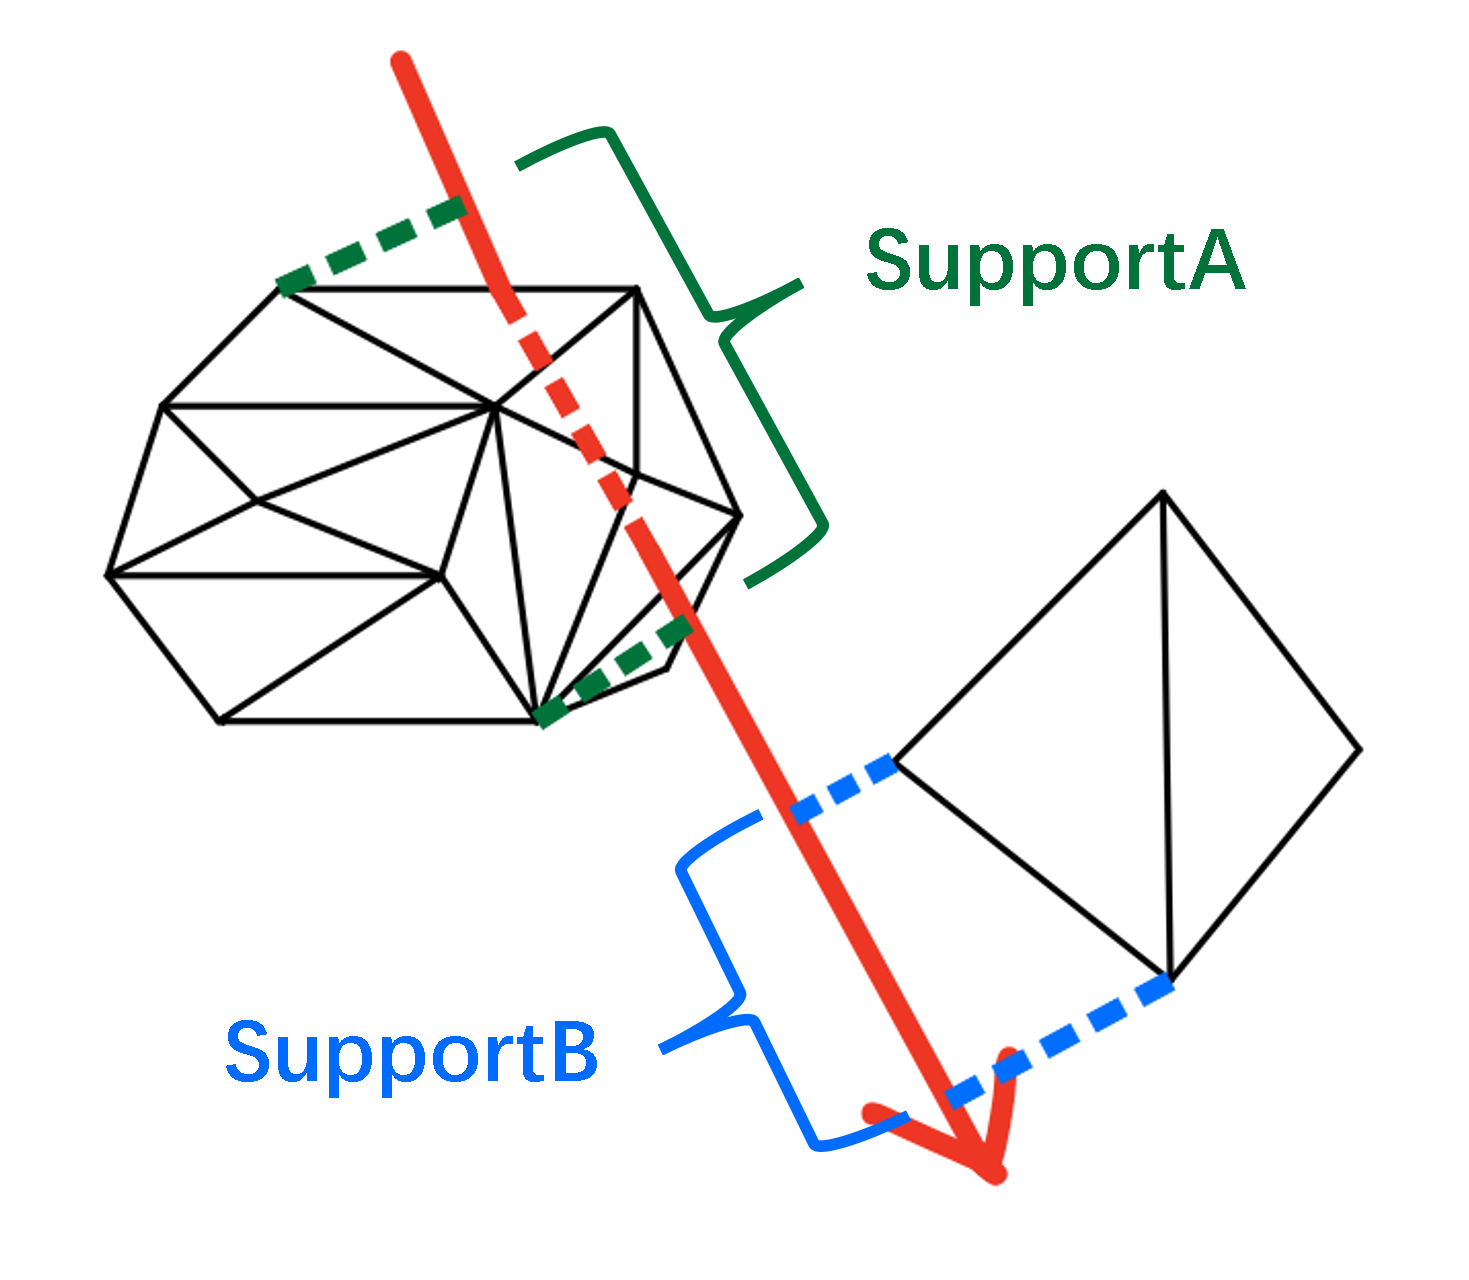
\includegraphics[scale=0.1]{sat algorithm.png}
		\caption{3D-SAT Algorithm}
		\label{fig:img4}
	\end{figure}

	
	\textbf{Main idea:} The separating axis theorem (SAT) says that: Two convex objects do not overlap if there exists a line (called axis) onto which the two objects' projections do not overlap. 
	
	\quad For example in Fig.\ref{fig:img4}, the two convex sets do not collide if and only if SupportA and SupportB do not intersect.
	
	\quad Let $C$ and $D$ be two convex sets in $R^n$ that do not intersect (i.e., $C\cap D=\emptyset$). Then, there exists $a\in R^n$, $a\not=0, b\in R$, such that $\forall x\in C,\forall y\in D$
	$$
	a^Tx\le b \text{ and } a^Ty\ge b
	$$
	
	As we talk in the related work part, we need carefully talk about boundaries cases. For two convex sets of intersecting polyhedra, the ways of intersecting them can be summarized as follows: f-f, f-e, f-v, e-e, e-v, v-v, where f is facet, e is edge, v is vertex. 
	
	\quad For the points in it, they can be treated as degenerate edges, so that the intersection between two convex sets can be simplified as: f-f, f-e, e-e.
	
	\quad For the above three simplified intersection ways, we can consider one by one to find all potential separation axes, so that we can get the potential separation plane between two convex sets may exist in the following positions:
	
	\begin{itemize}
		\item[1.] The plane of each polygon in A convex set A.
		
		\item[2.] The plane of each polygon in A convex set B.
		
		\item[3.]  The common vertical surface between each edge in convex set A and each edge in convex set B.

	\end{itemize}

	\quad And the direction of the corresponding separation axis is:
	
	\begin{itemize}
		\item[1.] The normal vector of each polygon in convex set A.
		
		\item[2.] The normal vector of each polygon in convex set B.
		
		\item[3.] The normal vector of the common vertical surface between every edge in convex set A and every edge in convex set B i.e. the cross product direction of the direction vectors of the two edges.
		
	\end{itemize}

	\begin{algorithm}
	\caption{3D-SAT algorithm}
	\begin{algorithmic}[2]
		\STATE // Get neccessary primitives
		\STATE verticesA, edgesA, normalsA $\leftarrow$ ConvexHullA
		\STATE verticesB, edgesB, normalsB $\leftarrow$ ConvexHullB
		\STATE // Choosing first normal set as axis
		\FOR{$n\leftarrow $ normalsA}
			\IF{!CheckSeprartingAxis(verticesA, verticesB, n)}
				\RETURN false // No collision !
			\ENDIF
		\ENDFOR
		\STATE // Choosing second normal set as axis
		\FOR{$n\leftarrow $ normalsB}
			\IF{!CheckSeprartingAxis(verticesA, verticesB, n)}
				\RETURN false // No collision !
			\ENDIF
		\ENDFOR
		\STATE Choosing cross product set by edges as axis
		\FOR{$e1 \leftarrow$ edgesA}
			\FOR{$e2 \leftarrow$ edgesB}
				\STATE axis $\leftarrow$ $e_1\times e_2$
				\IF{!CheckSeprartingAxis(verticesA, verticesB, axis)}
					\RETURN false // No collision !
				\ENDIF
			\ENDFOR
		\ENDFOR 
		\RETURN true // Collision detected!
	\end{algorithmic}
\end{algorithm}

\subsection*{How CheckSeparatingAxis works?}
		The function returns true if collision happens, false if not. In a short word, given a direction of axis, we perform the projection with the vertices on the convex hull, respectively. Then, we obtain two support regions.  
		
		\quad The collision happens if two support regions, in which case we should return true to continue searching for another potential axis.
		
\subsection*{Time complexity analysis}
	First, it takes $O(n)$ time to perform the initialization. 
	
	\quad Second, it takes $O(n)$ time to traverse all the normals of the convex hulls, and for each normal in convex hull, we need $O(n)$ time to perform the projection in order to check whether the collision happens. Thus, it takes $O(n^2)$ time to perform checking onto normals.

	\quad Third, we need perform projection along the direction of axis which is the cross product of edges in the first convex hull and the edges in the second convex hull. Thus, \# of axis w.r.t. edges is $O(n^2)$, and for each axis, we need perform projection in $O(n)$ time. Thus, the time complexity of edges cases need $O(n^3)$ time complexity, which becomes our 3D-SAT algorithm's bottleneck. 
	
	\quad To sum up, the total time complexity is $O(n^3)$.
\subsection*{SpeedUp}
	\qquad Thanks to the power of OpenMP, we can speed up this process about $10$ times, which gives us a tolerable time complexity.
	
\section{Results}
	We support two kinds of geometry for convex hull construction and collision detected, that from obj file or generating randomly within sphere.
\subsection{Bunny cases}

\begin{figure}[htbp]
	\centering
	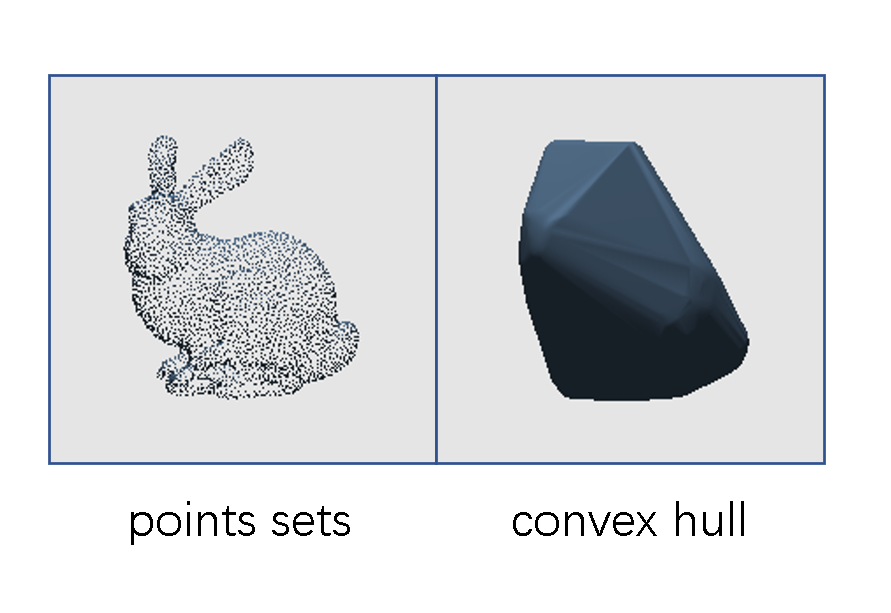
\includegraphics[scale=0.2]{scene0.png}
	\caption{Scene0: one bunny}
	\label{fig:0}
\end{figure}

\begin{figure}[htbp]
	\centering
	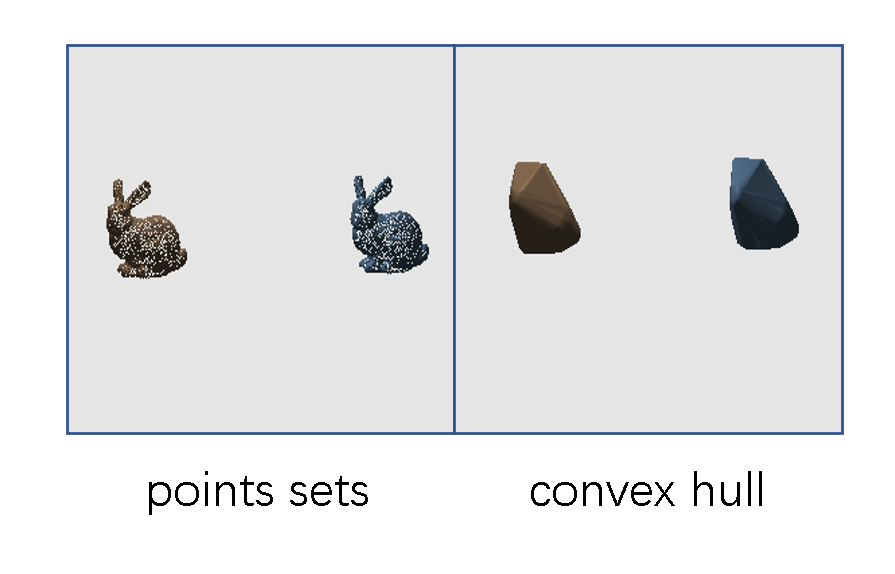
\includegraphics[scale=0.2]{scene1.png}
	\caption{Scene1: two bunny and no collision}
	\label{fig:1}
\end{figure}

\begin{figure}[htbp]
	\centering
	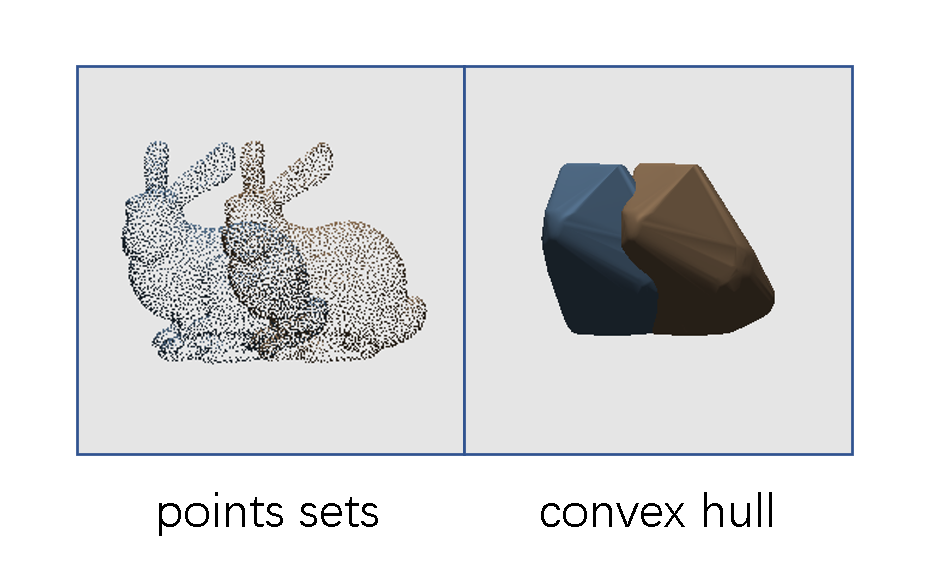
\includegraphics[scale=0.2]{scene2.png}
	\caption{Scene2: two bunny and collision obviously}
	\label{fig:2}
\end{figure}

\begin{figure}[htbp]
	\centering
	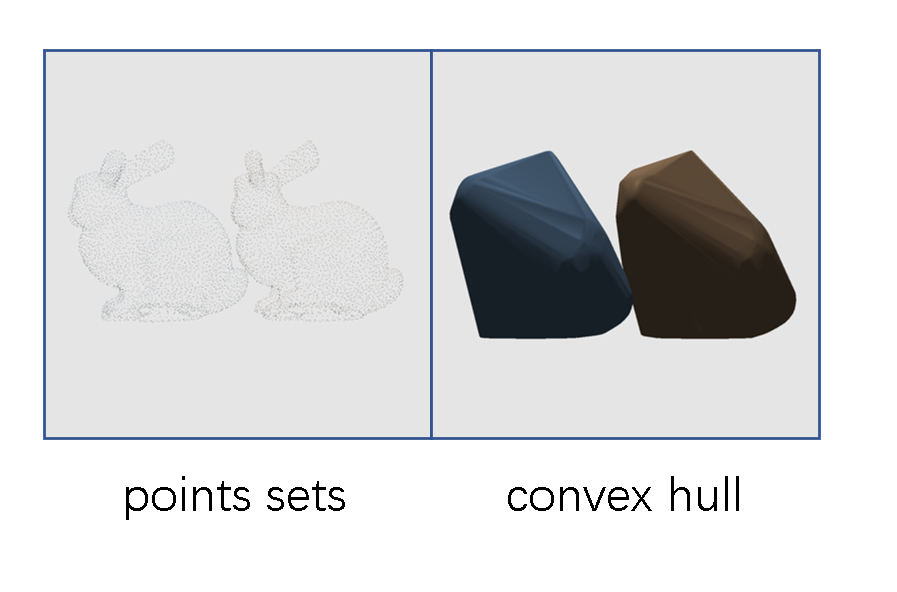
\includegraphics[scale=0.2]{scene3.png}
	\caption{Scene3: two bunny and collision unobviously}
	\label{fig:3}
\end{figure}

\begin{figure}[htbp]
	\centering
	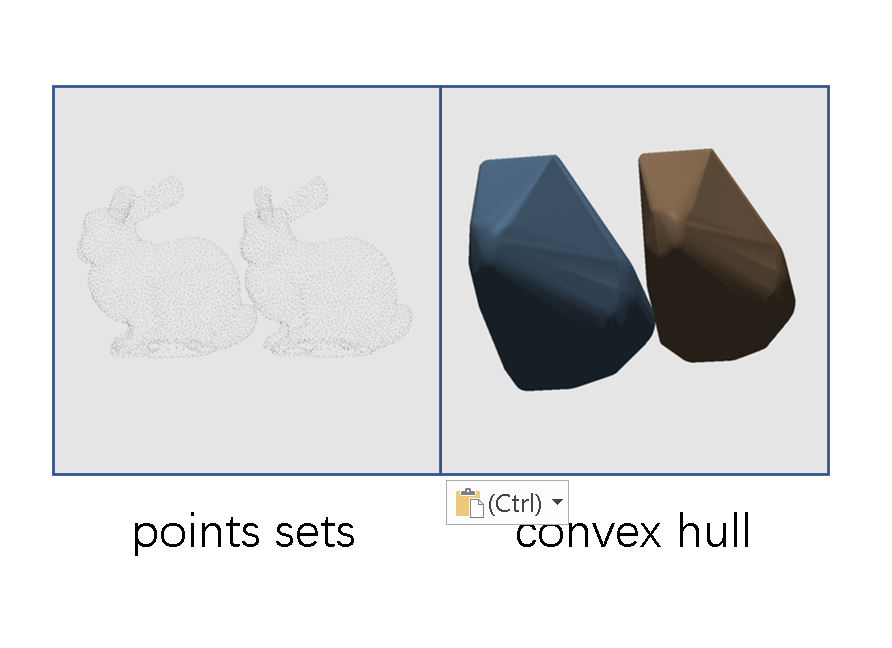
\includegraphics[scale=0.2]{scene4.png}
	\caption{Scene 4: two bunny and collision boundary}
	\label{fig:4}
\end{figure}

\subsection{Sphere cases}


\begin{figure}[htbp]
	\centering
	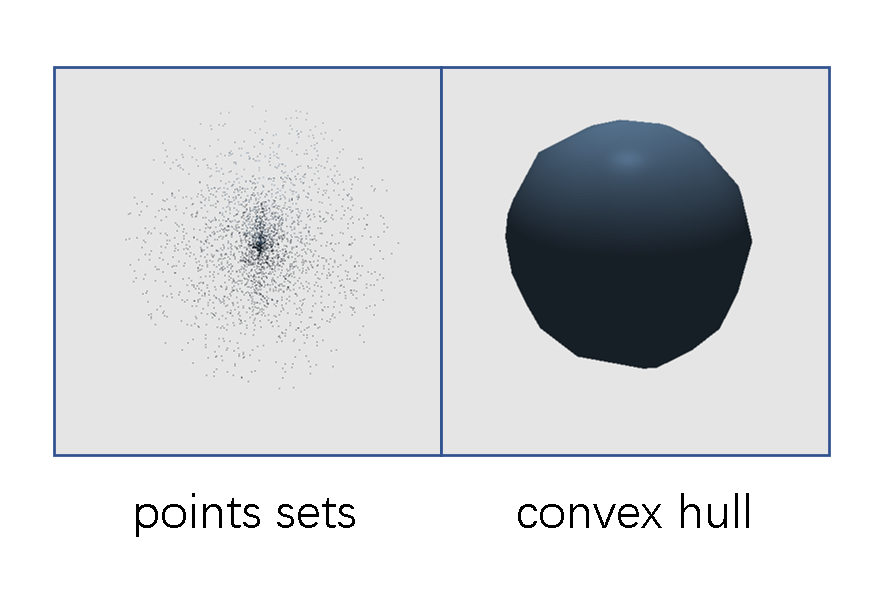
\includegraphics[scale=0.2]{scene5.png}
	\caption{Scene5: 3000 random samples within sphere}
	\label{fig:5}
\end{figure}

\begin{figure}[htbp]
	\centering
	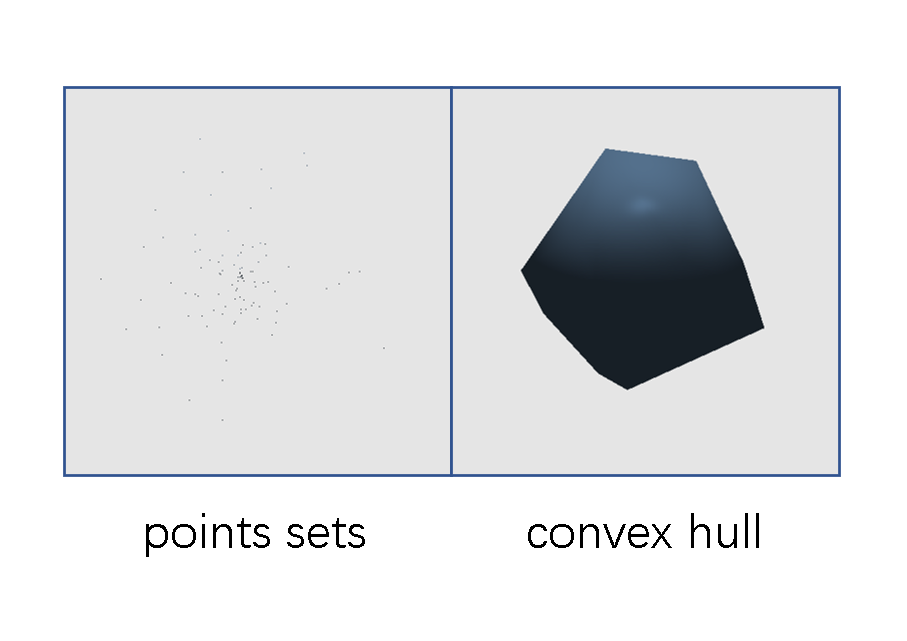
\includegraphics[scale=0.2]{scene6.png}
	\caption{Scene6: 100 randoms samples within sphere}
	\label{fig:6}
\end{figure}

\begin{figure}[htbp]
	\centering
	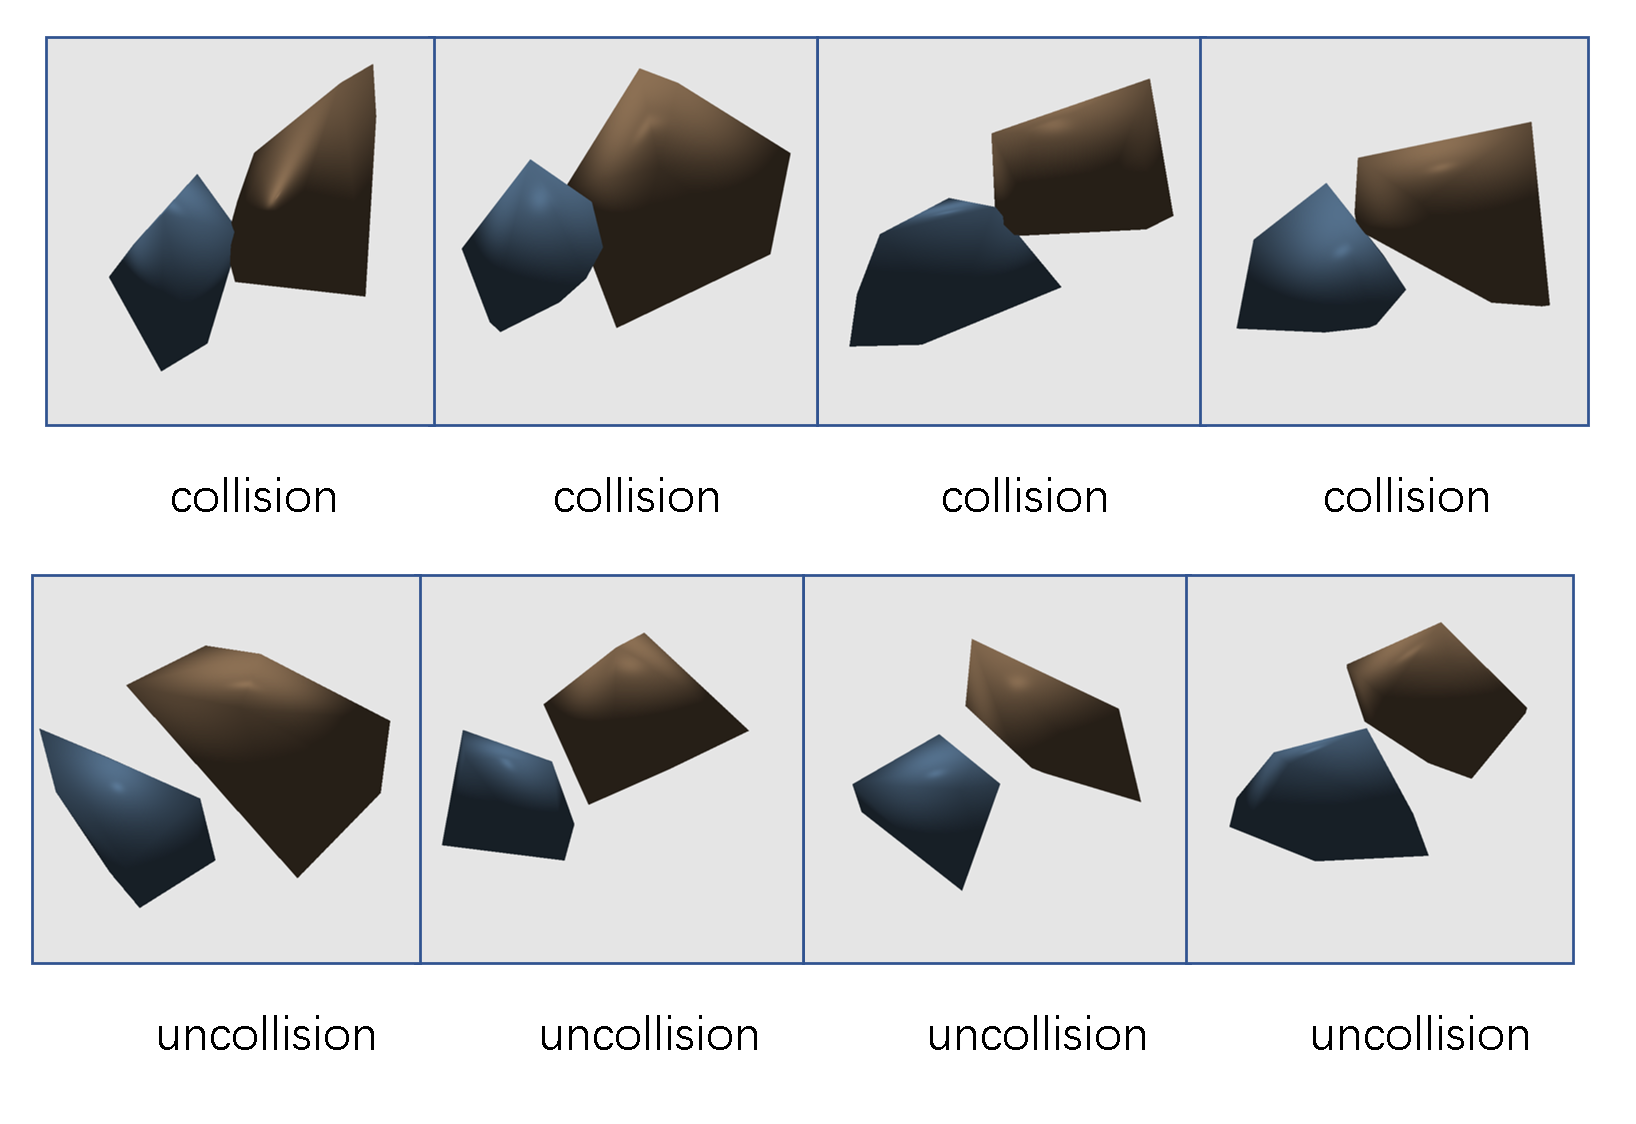
\includegraphics[scale=0.15]{scene7.png}
	\caption{Scene7: two spheres randomly}
	\label{fig:7}
\end{figure}

\end{document}
